\documentclass[conference]{IEEEtran}
\IEEEoverridecommandlockouts

\usepackage{cite}
\usepackage{amsmath,amssymb,amsfonts}
\usepackage{graphicx}
\usepackage{textcomp}
\usepackage{xcolor}
\usepackage{booktabs}
\usepackage{multirow}
\usepackage{url}
\usepackage{hyperref}
\hypersetup{colorlinks=true, linkcolor=blue, citecolor=blue, urlcolor=blue}

\graphicspath{{outputs/}}

\def\BibTeX{{\rm B\kern-.05em{\sc i\kern-.025em b}\kern-.08em
    T\kern-.1667em\lower.7ex\hbox{E}\kern-.125emX}}

\begin{document}

\title{All-in-Focus Reconstruction from Focal Stacks\\
\large{A Classical Computational Imaging Study on Macro-Style Photography}}

\author{
  \IEEEauthorblockN{Engin Samet Dede}
  \IEEEauthorblockA{Computational Imaging Mini-Project\\
  May 2026}
}

\maketitle

%------------------------------------------------------------
\begin{abstract}
Shallow depth of field in macro and close-up photography prevents any single image from rendering the entire subject in focus. Focal-stack fusion addresses this by combining a sequence of images that each focus on a different depth plane into one all-in-focus composite. This work implements and evaluates the complete focal-stack pipeline—image loading, ECC-based alignment, focus measure computation, focus map construction, and multi-scale fusion—on four datasets of increasing realism: a 23-frame plants baseline, a personal 6-frame flower macro stack, a 3-frame insect stack captured in the field, and pre-registered Lytro two-focus pairs. Four focus measures (Laplacian variance, Tenengrad energy, local contrast, and Sum-Modified Laplacian) are compared systematically, and three fusion strategies (winner-takes-all, soft/softmax blending, and Laplacian pyramid fusion) are evaluated using Tenengrad sharpness, SSIM, and Shannon entropy. Tenengrad consistently ranks first across all datasets; WTA fusion achieves the highest sharpness gain while pyramid blending best preserves structural similarity.
\end{abstract}

\begin{IEEEkeywords}
focal stack, all-in-focus reconstruction, focus measure, image fusion, Laplacian pyramid, depth of field, macro photography
\end{IEEEkeywords}

%------------------------------------------------------------
\section{Introduction}

Macro photography reveals fine structure in small subjects—insects, flowers, circuit traces—at working distances where the effective depth of field (DoF) can be less than a millimeter. Within this regime no single exposure keeps the full subject sharp; parts nearer or farther from the focal plane appear blurred regardless of aperture. Specialized techniques such as focus-bracketed shooting and computational fusion allow a photographer to combine multiple exposures into an all-in-focus image without physically altering the optical system.

The motivating scenario for this project is macro insect photography captured with a smartphone camera (Apple iPhone 17 Pro Max, ProRAW mode). The phone's primary lens operates at a fixed aperture of $f/1.78$ with a 6.765\,mm focal length, giving a very shallow DoF at close range. Dedicated macro lenses or extension tubes are not required; instead, a short burst of images with refocused depth planes is post-processed computationally.

This report makes the following contributions:
\begin{itemize}
  \item A complete, end-to-end focal-stack pipeline implemented in Python (NumPy, OpenCV, SciPy) without any deep-learning framework for the core method.
  \item A systematic comparison of four focus measures on two independent datasets (plants and Lytro), demonstrating that the method ranking is consistent across domains.
  \item Application of the pipeline to personal close-up stacks (flower and insect) captured with a smartphone.
  \item An optional tiny learned focus-scorer (pure NumPy MLP) as an exploratory extension.
\end{itemize}

%------------------------------------------------------------
\section{Related Work}

Focal-stack fusion has been studied extensively in computational photography. The foundational approach of \emph{winner-takes-all} (WTA) pixel selection based on local sharpness was described by Nayar and Nakagawa~\cite{nayar1994shape}. Laplacian-based focus measures were introduced by Krotkov~\cite{krotkov1988focusing} and refined by Pertuz et al.\ who systematically benchmarked over 30 focus measures~\cite{pertuz2013analysis}. The Tenengrad criterion, based on Sobel gradient energy, was shown to be among the most robust under noise~\cite{santos1997evaluation}. The selection of an optimal focus measure for depth-from-focus was studied by Subbarao and Tyan~\cite{subbarao1998optimal}, who showed that measures based on gradient energy generalise better across textures than Laplacian-based ones.

Laplacian pyramid blending for seamless multi-focus fusion was proposed by Burt and Adelson~\cite{burt1983multiresolution}. Zhang and Blum provide a thorough categorisation of multi-scale decomposition fusion schemes and a practical performance study for digital-camera applications~\cite{zhang1999categorization}. More recently, Liu et al.\ demonstrated that deep convolutional features can replace hand-crafted focus measures for multi-focus fusion, achieving sharper composites on benchmark datasets~\cite{liu2017multifocus}. The Lytro two-focus benchmark dataset used in this work was introduced by Nejati et al.~\cite{nejati2015multi}. ECC-based image alignment~\cite{evangelidis2008parametric} is used to register handheld stacks before fusion; a comprehensive treatment of image registration and alignment is given in Szeliski~\cite{szeliski2010}.

%------------------------------------------------------------
\section{Methods}

\subsection{Pipeline Overview}

The pipeline has five stages: (1) load and optionally resize each frame, (2) align frames with ECC for handheld stacks, (3) compute a per-pixel focus score for each frame, (4) build a focus map, and (5) fuse the stack. Table~\ref{tab:hyperparams} lists all fixed hyperparameters.

\begin{table}[h]
\centering
\caption{Pipeline hyperparameters used throughout all experiments.}
\label{tab:hyperparams}
\begin{tabular}{lll}
\toprule
Parameter & Value & Role \\
\midrule
Focus measure         & Tenengrad   & Primary scoring method \\
Averaging window $W$  & $17\times17$& Local score smoothing \\
Median filter         & $5\times5$  & Focus map denoising \\
Softmax temperature $\beta$ & 8   & Soft/pyramid weight sharpness \\
Pyramid levels $L$    & 5           & Laplacian pyramid depth \\
Max long edge         & 1920\,px    & Downsampling limit \\
ECC max iterations    & 100         & Alignment convergence \\
ECC threshold         & $10^{-5}$   & Alignment stopping criterion \\
\bottomrule
\end{tabular}
\end{table}

\subsection{Focus Measures}

Let $G_k$ denote the grayscale version of frame $k$ in the stack. Four focus measures are implemented.

\textbf{Laplacian variance.}
\begin{equation}
  S_k^{\text{Lap}}(p) = \bigl[\nabla^2 G_k(p)\bigr]^2
\end{equation}
The squared Laplacian response captures second-order intensity variation at each pixel. A local average over a $W\!\times\!W$ window gives the spatially smoothed score used in the focus map.

\textbf{Tenengrad (Sobel energy).}
\begin{equation}
  S_k^{\text{Ten}}(p) = \bigl[G_x^k(p)\bigr]^2 + \bigl[G_y^k(p)\bigr]^2
\end{equation}
where $G_x^k$ and $G_y^k$ are the horizontal and vertical Sobel responses of frame $k$. This measure is robust to noise and is the primary method used throughout the project.

\textbf{Local contrast.}
\begin{equation}
  S_k^{\text{LC}}(p) = \bigl[G_k(p) - \mu_k^W(p)\bigr]^2
\end{equation}
where $\mu_k^W$ is a local mean over a $W\!\times\!W$ neighbourhood. This is computationally inexpensive but less discriminative near uniform regions.

\textbf{Sum-Modified Laplacian (SML).}
\begin{equation}
  \text{ML}(p) = |2G(p) - G(p\!-\!\delta) - G(p\!+\!\delta)|
\end{equation}
applied separately in horizontal and vertical directions with step $\delta=2$ and summed~\cite{nayar1994shape,subbarao1998optimal}. The SML avoids cancellation of opposing Laplacian signs that arises when positive and negative second-derivative responses cancel in the standard Laplacian.

All focus score volumes are spatially smoothed by a $17\!\times\!17$ local average and then median-filtered (size 5) to reduce salt-and-pepper artefacts in the focus map.

\subsection{Focus Map Construction}

The focus map $F(p) \in \{0,\ldots,N-1\}$ assigns each pixel to the frame with the highest local focus score:
\begin{equation}
  F(p) = \arg\max_{k}\, S_k(p)
\end{equation}

\subsection{Fusion Strategies}

\textbf{Winner-Takes-All (WTA).}
Each output pixel is taken directly from the frame indicated by the focus map:
\begin{equation}
  I^{\text{WTA}}(p) = I_{F(p)}(p)
\end{equation}
This maximises sharpness but can introduce sharp transition artefacts at focus-map boundaries.

\textbf{Soft (softmax) fusion.}
Per-frame weights are computed via a temperature-scaled softmax over the focus scores:
\begin{equation}
  w_k(p) = \frac{\exp\!\bigl(\beta\,\tilde{S}_k(p)\bigr)}{\sum_j \exp\!\bigl(\beta\,\tilde{S}_j(p)\bigr)}
\end{equation}
where $\tilde{S}_k = S_k - \max_j S_j$ (for numerical stability) and $\beta=8$. The fused image is $I^{\text{Soft}} = \sum_k w_k \odot I_k$. This produces smooth spatial transitions at the cost of slightly reduced peak sharpness.

\textbf{Laplacian pyramid blending.}
For each frame $k$ and its corresponding softmax weight map $w_k$, Laplacian pyramids of the frame and Gaussian pyramids of the weight are computed to $L=5$ levels. The pyramids are blended level by level and collapsed to produce the fused output~\cite{burt1983multiresolution,zhang1999categorization}. This strategy preserves both sharpness and structural continuity.

\subsection{ECC Alignment}

For handheld stacks the camera moves slightly between exposures, producing misregistration that creates ghosting in the fused output. Enhanced Correlation Coefficient (ECC) optimization~\cite{evangelidis2008parametric} is used to estimate a translation warp for each frame relative to the first, using 100 iterations and a convergence threshold of $10^{-5}$.

\subsection{Quality Metrics}

Three metrics evaluate fusion quality:
\begin{itemize}
  \item \textbf{Tenengrad sharpness}: global mean Sobel energy of the fused image; higher is sharper~\cite{santos1997evaluation}.
  \item \textbf{SSIM}~\cite{wang2004ssim}: structural similarity index to the reference frame (sharpest single frame); higher means more structural content preserved. The index jointly measures luminance, contrast, and structure.
  \item \textbf{Shannon entropy}~\cite{shannon1948}: $H = -\sum_i p_i \log_2 p_i$ of the grayscale histogram; higher means a richer intensity distribution and more textural detail.
\end{itemize}

%------------------------------------------------------------
\section{Experimental Setup}

\subsection{Datasets}

Table~\ref{tab:datasets} summarises all datasets used in this study.

\begin{table}[h]
\centering
\caption{Dataset summary.}
\label{tab:datasets}
\resizebox{\columnwidth}{!}{%
\begin{tabular}{llccl}
\toprule
Dataset   & Source        & Frames & Resolution      & Alignment \\
\midrule
Plants    & Public        & 23     & $360\times640$  & None (tripod) \\
Flower    & iPhone ProRAW &  6     & $1920\times1440$& ECC \\
Insect    & iPhone ProRAW &  3     & $1920\times1380$& ECC \\
Lytro-03  & Nejati et al.~\cite{nejati2015multi} & 2 & $520\times520$ & None (pre-registered) \\
Lytro-11  & Nejati et al.~\cite{nejati2015multi} & 2 & $520\times520$ & None (pre-registered) \\
Lytro-13  & Nejati et al.~\cite{nejati2015multi} & 2 & $520\times520$ & None (pre-registered) \\
\bottomrule
\end{tabular}%
}
\end{table}

\textbf{Plants (baseline).} A publicly available 23-frame focal stack of potted plants. No alignment is applied. This dataset serves as the primary benchmark for method selection.

\textbf{Flower stack.} Six ProRAW frames ($f/1.78$, 6.765\,mm) of a flower captured with an iPhone 17 Pro Max on 23 May 2026. Images were converted from HEIC to JPEG via \texttt{sips} with EXIF-rotation correction ($-$90\,CW), then downsampled to 1920\,px on the long edge. ECC alignment is applied.

\textbf{Insect stack.} Three frames of the same insect (IMG\_6887, IMG\_6888, IMG\_6889), captured hand-held. IMG\_6887 and IMG\_6889 carried EXIF ``Rotate 90 CW'' tags and required pixel-level rotation. IMG\_6888 had a different native width (2900\,px vs.\ 3024\,px), resolved by center-cropping all frames to the smallest common width before stacking. ECC alignment is applied.

\textbf{Lytro benchmark.} Three pre-registered two-focus pairs from Nejati et al.~\cite{nejati2015multi}: lytro-03 (child and toy), lytro-11 (camera and globe), lytro-13 (zoo sign and tigers). No alignment is applied; these serve as an independent cross-domain validation of the selected focus measure.

\subsection{Implementation}

All code is written in Python using NumPy, OpenCV, SciPy, and Matplotlib. The pipeline runs in a Jupyter notebook without any deep-learning framework. Images are loaded as float32 in $[0,1]$. Outputs are saved as PNG.

%------------------------------------------------------------
\section{Results and Discussion}

\subsection{Focus Measure Comparison}

Table~\ref{tab:method_comparison} shows the WTA-fused Tenengrad sharpness for all four methods on the plants stack (window $W=17$) and the average over three Lytro pairs.

\begin{table}[h]
\centering
\caption{Focus measure comparison: WTA-fused Tenengrad sharpness and ranking on two independent datasets.}
\label{tab:method_comparison}
\begin{tabular}{lcccc}
\toprule
Method & Plants & Lytro avg & Rank (P) & Rank (L) \\
\midrule
Laplacian  & 0.1039 & 0.3469 & \#3 & \#3 \checkmark \\
Tenengrad  & \textbf{0.1049} & \textbf{0.3473} & \#1 & \#1 \checkmark \\
Contrast   & 0.1031 & 0.3468 & \#4 & \#4 \checkmark \\
SML        & 0.1045 & 0.3470 & \#2 & \#2 \checkmark \\
\bottomrule
\end{tabular}
\end{table}

The ranking is \emph{identical} on both datasets (Tenengrad $>$ SML $>$ Laplacian $>$ Contrast), confirming that the selection made on the plants baseline generalises to the independent Lytro benchmark. The numerical differences are small ($<$2\% between Tenengrad and SML), consistent with prior findings that gradient-energy measures form a close cluster~\cite{pertuz2013analysis}. Tenengrad is selected as the primary method throughout.

\subsection{Plants Dataset: Full Pipeline}

Fig.~\ref{fig:plants} shows the plants dataset results. The focus map correctly identifies the depth-ordered zones across the 23-frame stack: nearby leaves are highlighted by low-index frames, farther background regions by higher-index frames.

\begin{figure*}[t]
\centering
\begin{minipage}{0.24\textwidth}
  \centering
  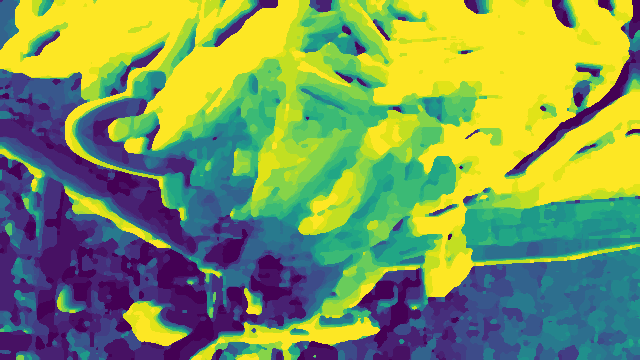
\includegraphics[width=\linewidth]{focus_map.png}
  \caption*{(a) Focus map}
\end{minipage}\hfill
\begin{minipage}{0.24\textwidth}
  \centering
  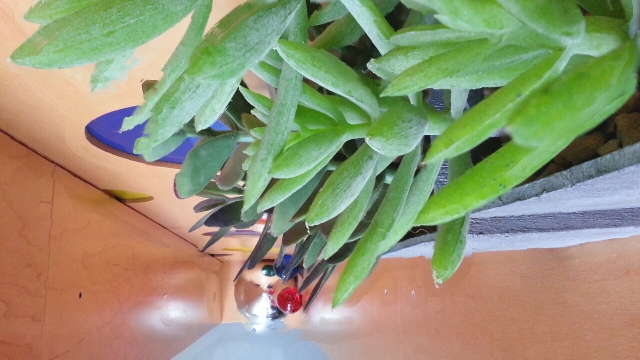
\includegraphics[width=\linewidth]{fused_winner_takes_all.png}
  \caption*{(b) Winner-Takes-All}
\end{minipage}\hfill
\begin{minipage}{0.24\textwidth}
  \centering
  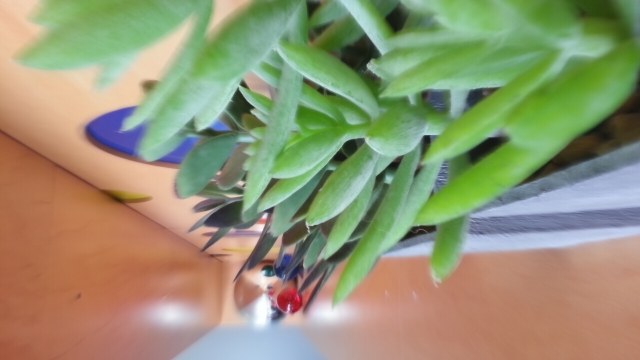
\includegraphics[width=\linewidth]{fused_soft.png}
  \caption*{(c) Soft (softmax)}
\end{minipage}\hfill
\begin{minipage}{0.24\textwidth}
  \centering
  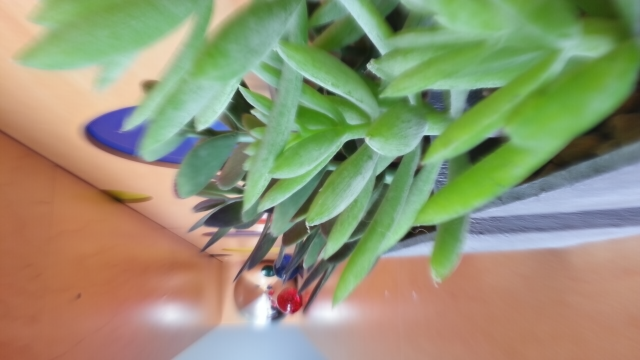
\includegraphics[width=\linewidth]{fused_pyramid.png}
  \caption*{(d) Laplacian pyramid}
\end{minipage}
\caption{Plants baseline: focus map and three fused outputs. WTA produces the sharpest composite (Tenengrad: 0.105); soft and pyramid blending yield higher SSIM at the cost of some peak sharpness.}
\label{fig:plants}
\end{figure*}

\subsection{Fusion Strategy Comparison}

Table~\ref{tab:fusion_metrics} reports all three metrics for each fusion strategy across all datasets.

\begin{table*}[t]
\centering
\caption{Fusion quality metrics across all datasets. Ten = Tenengrad sharpness; best value per metric per dataset is bold.}
\label{tab:fusion_metrics}
\begin{tabular}{llcccccc}
\toprule
 & & \multicolumn{3}{c}{Personal stacks} & \multicolumn{3}{c}{Lytro benchmark} \\
\cmidrule(lr){3-5}\cmidrule(lr){6-8}
Dataset & Method & Ten & SSIM & Entropy & Ten & SSIM & Entropy \\
\midrule
\multirow{4}{*}{Plants}
  & Sharpest frame & 0.0778 & 1.000 & 7.213 & -- & -- & -- \\
  & WTA            & \textbf{0.1049} & 0.764 & 7.237 & -- & -- & -- \\
  & Soft           & 0.0552 & 0.902 & 7.167 & -- & -- & -- \\
  & Pyramid        & 0.0555 & \textbf{0.903} & 7.173 & -- & -- & -- \\
\midrule
\multirow{4}{*}{Flower}
  & Sharpest frame & 0.0698 & 1.000 & 7.567 & -- & -- & -- \\
  & WTA            & \textbf{0.2322} & 0.413 & 7.619 & -- & -- & -- \\
  & Soft           & 0.0711 & 0.589 & 7.516 & -- & -- & -- \\
  & Pyramid        & 0.0515 & \textbf{0.605} & 7.488 & -- & -- & -- \\
\midrule
\multirow{4}{*}{Insect}
  & Sharpest frame & 0.0569 & 1.000 & 7.531 & -- & -- & -- \\
  & WTA            & \textbf{0.1276} & 0.649 & 7.603 & -- & -- & -- \\
  & Soft           & 0.0456 & 0.673 & 7.403 & -- & -- & -- \\
  & Pyramid        & 0.0397 & \textbf{0.680} & 7.416 & -- & -- & -- \\
\midrule
\multirow{4}{*}{Lytro-03}
  & Sharpest frame & -- & -- & -- & 0.0919 & 1.000 & 7.497 \\
  & WTA            & -- & -- & -- & \textbf{0.1246} & 0.836 & 7.527 \\
  & Soft           & -- & -- & -- & 0.0991 & 0.883 & 7.506 \\
  & Pyramid        & -- & -- & -- & 0.0987 & \textbf{0.883} & 7.506 \\
\midrule
\multirow{4}{*}{Lytro-11}
  & Sharpest frame & -- & -- & -- & 0.4318 & 1.000 & 7.720 \\
  & WTA            & -- & -- & -- & \textbf{0.4658} & 0.953 & 7.721 \\
  & Soft           & -- & -- & -- & 0.4532 & 0.961 & 7.722 \\
  & Pyramid        & -- & -- & -- & 0.4529 & \textbf{0.961} & 7.730 \\
\midrule
\multirow{4}{*}{Lytro-13}
  & Sharpest frame & -- & -- & -- & 0.3676 & 1.000 & 7.631 \\
  & WTA            & -- & -- & -- & \textbf{0.4515} & 0.847 & 7.630 \\
  & Soft           & -- & -- & -- & 0.4235 & 0.871 & 7.622 \\
  & Pyramid        & -- & -- & -- & 0.4228 & \textbf{0.872} & 7.621 \\
\bottomrule
\end{tabular}
\end{table*}

\textbf{Sharpness gain.} Table~\ref{tab:gain} summarises the absolute Tenengrad improvement from WTA fusion over the best single frame. Personal stacks benefit far more than the Lytro pairs because the former have larger focal separation between frames; Lytro-11 already has high native contrast.

\begin{table}[h]
\centering
\caption{WTA Tenengrad sharpness gain over the best single frame.}
\label{tab:gain}
\begin{tabular}{lccc}
\toprule
Dataset   & Single frame & WTA    & Gain \\
\midrule
Plants    & 0.0778 & 0.1049 & $+$35\% \\
Flower    & 0.0698 & 0.2322 & $+$233\% \\
Insect    & 0.0569 & 0.1276 & $+$124\% \\
Lytro-03  & 0.0919 & 0.1246 & $+$36\% \\
Lytro-11  & 0.4318 & 0.4658 & $+$8\%  \\
Lytro-13  & 0.3676 & 0.4515 & $+$23\% \\
\bottomrule
\end{tabular}
\end{table}

\textbf{SSIM vs.\ sharpness trade-off.} WTA consistently yields the highest Tenengrad score but the lowest SSIM because hard pixel-switching introduces spatial discontinuities at focus-map boundaries. Soft and pyramid blending sacrifice some peak sharpness in exchange for smoother transitions and higher structural fidelity.

\textbf{Pyramid vs.\ soft.} The two methods produce nearly identical SSIM and entropy in most cases, with pyramid blending edging ahead slightly (e.g., Lytro-13: SSIM 0.872 vs.\ 0.871). This marginal difference is consistent with theory: pyramid blending explicitly decorrelates artefacts across frequency bands, but on low-resolution stacks ($520\!\times\!520$) the advantage is small.

\subsection{Flower Stack Results}

The flower stack provides the largest sharpness gain of any dataset (+233\%), reflecting the wide focal sweep across the six frames. Fig.~\ref{fig:flower} shows the focus map and fused outputs.

\begin{figure*}[t]
\centering
\begin{minipage}{0.24\textwidth}
  \centering
  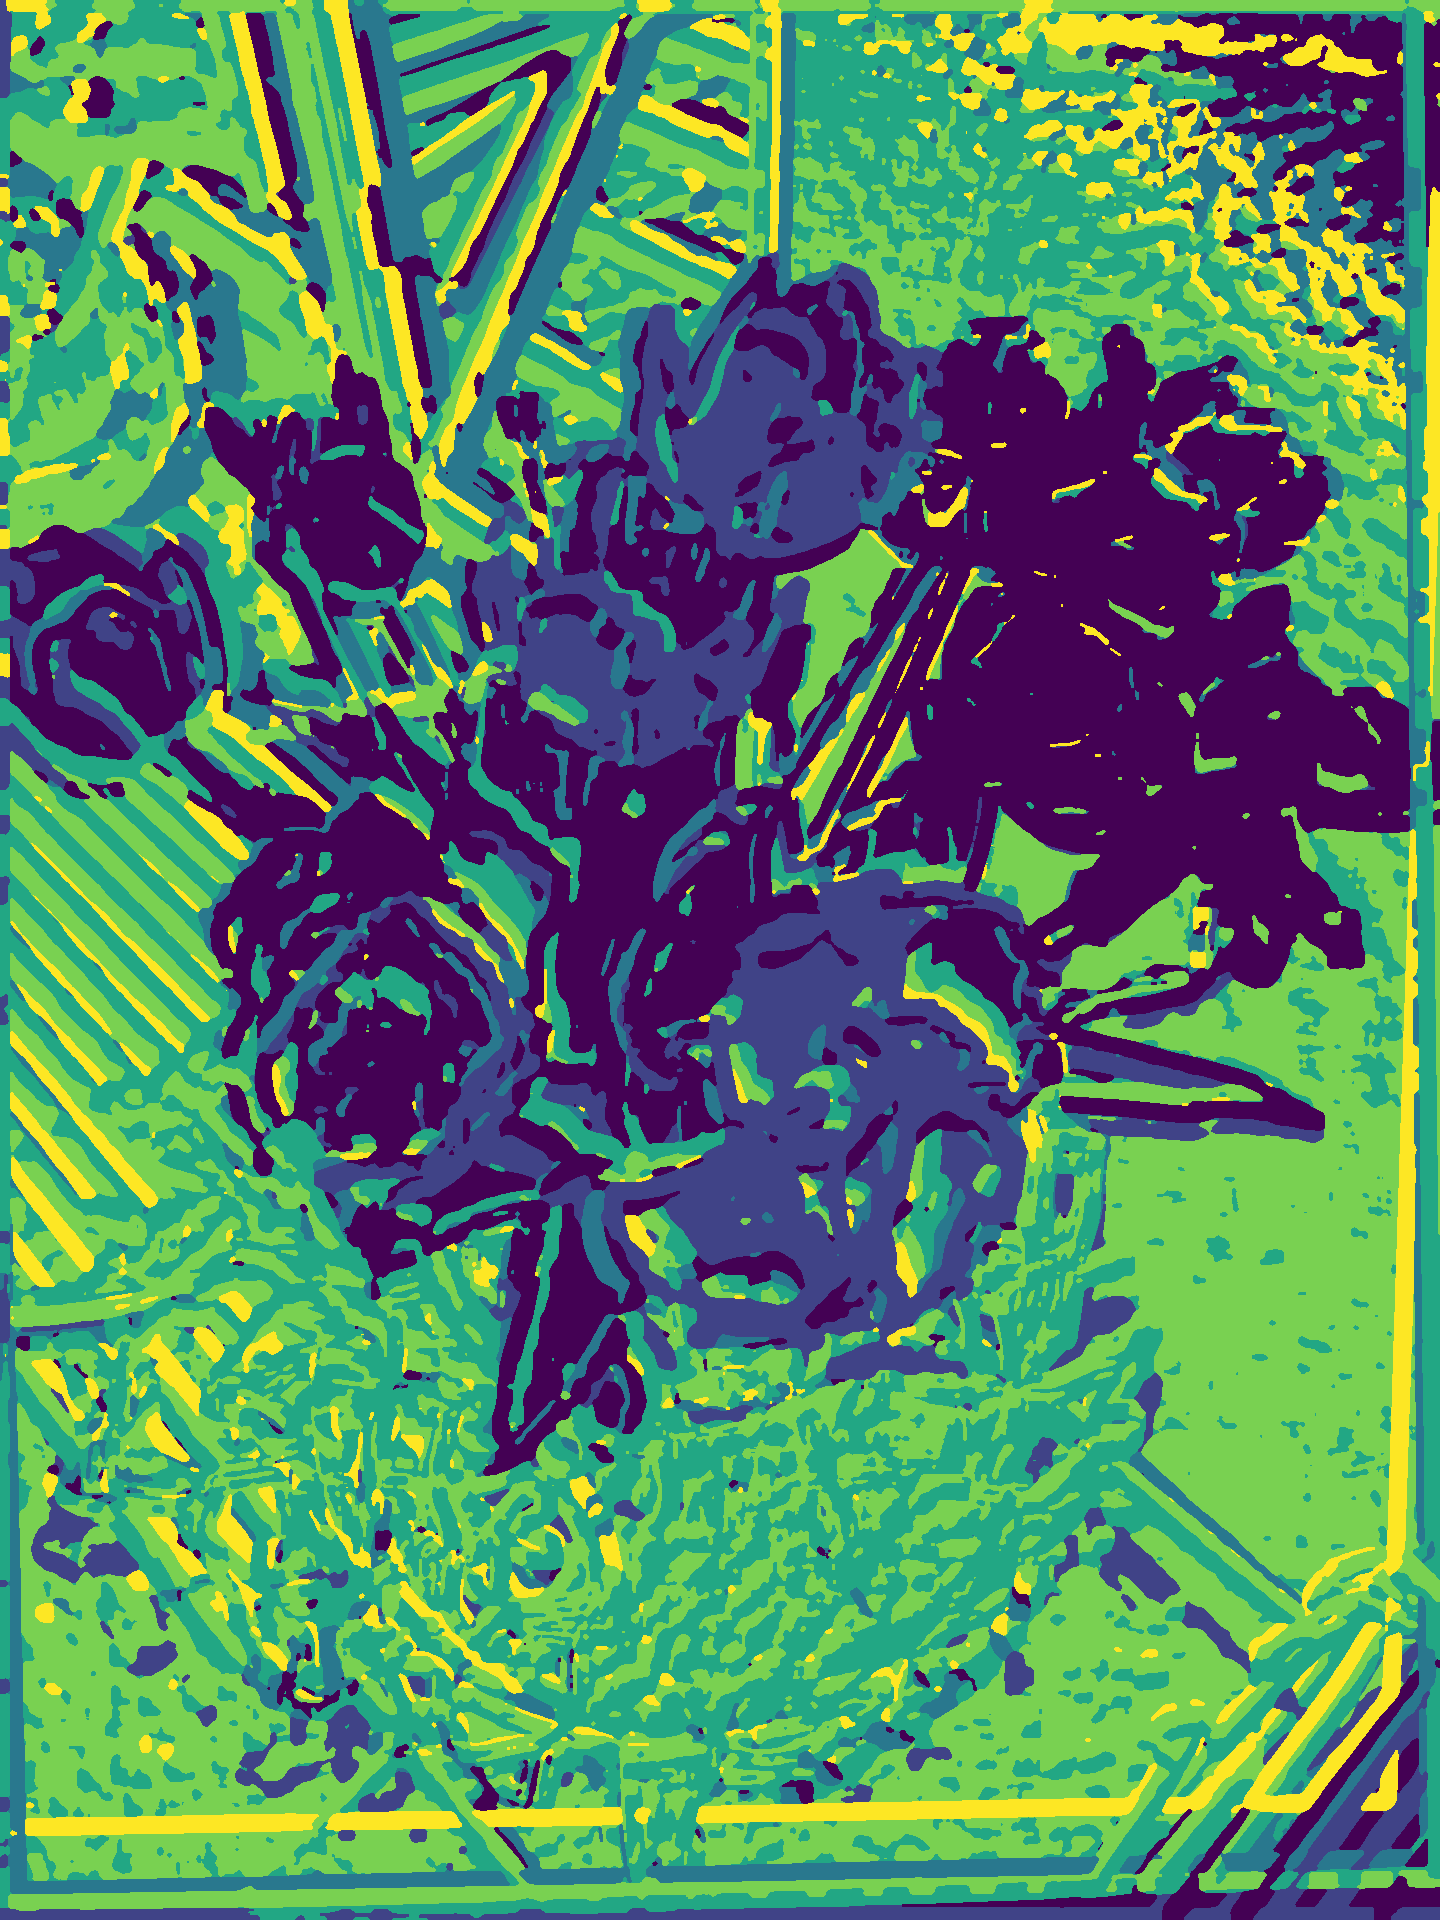
\includegraphics[width=\linewidth]{flower_focus_map.png}
  \caption*{(a) Focus map}
\end{minipage}\hfill
\begin{minipage}{0.24\textwidth}
  \centering
  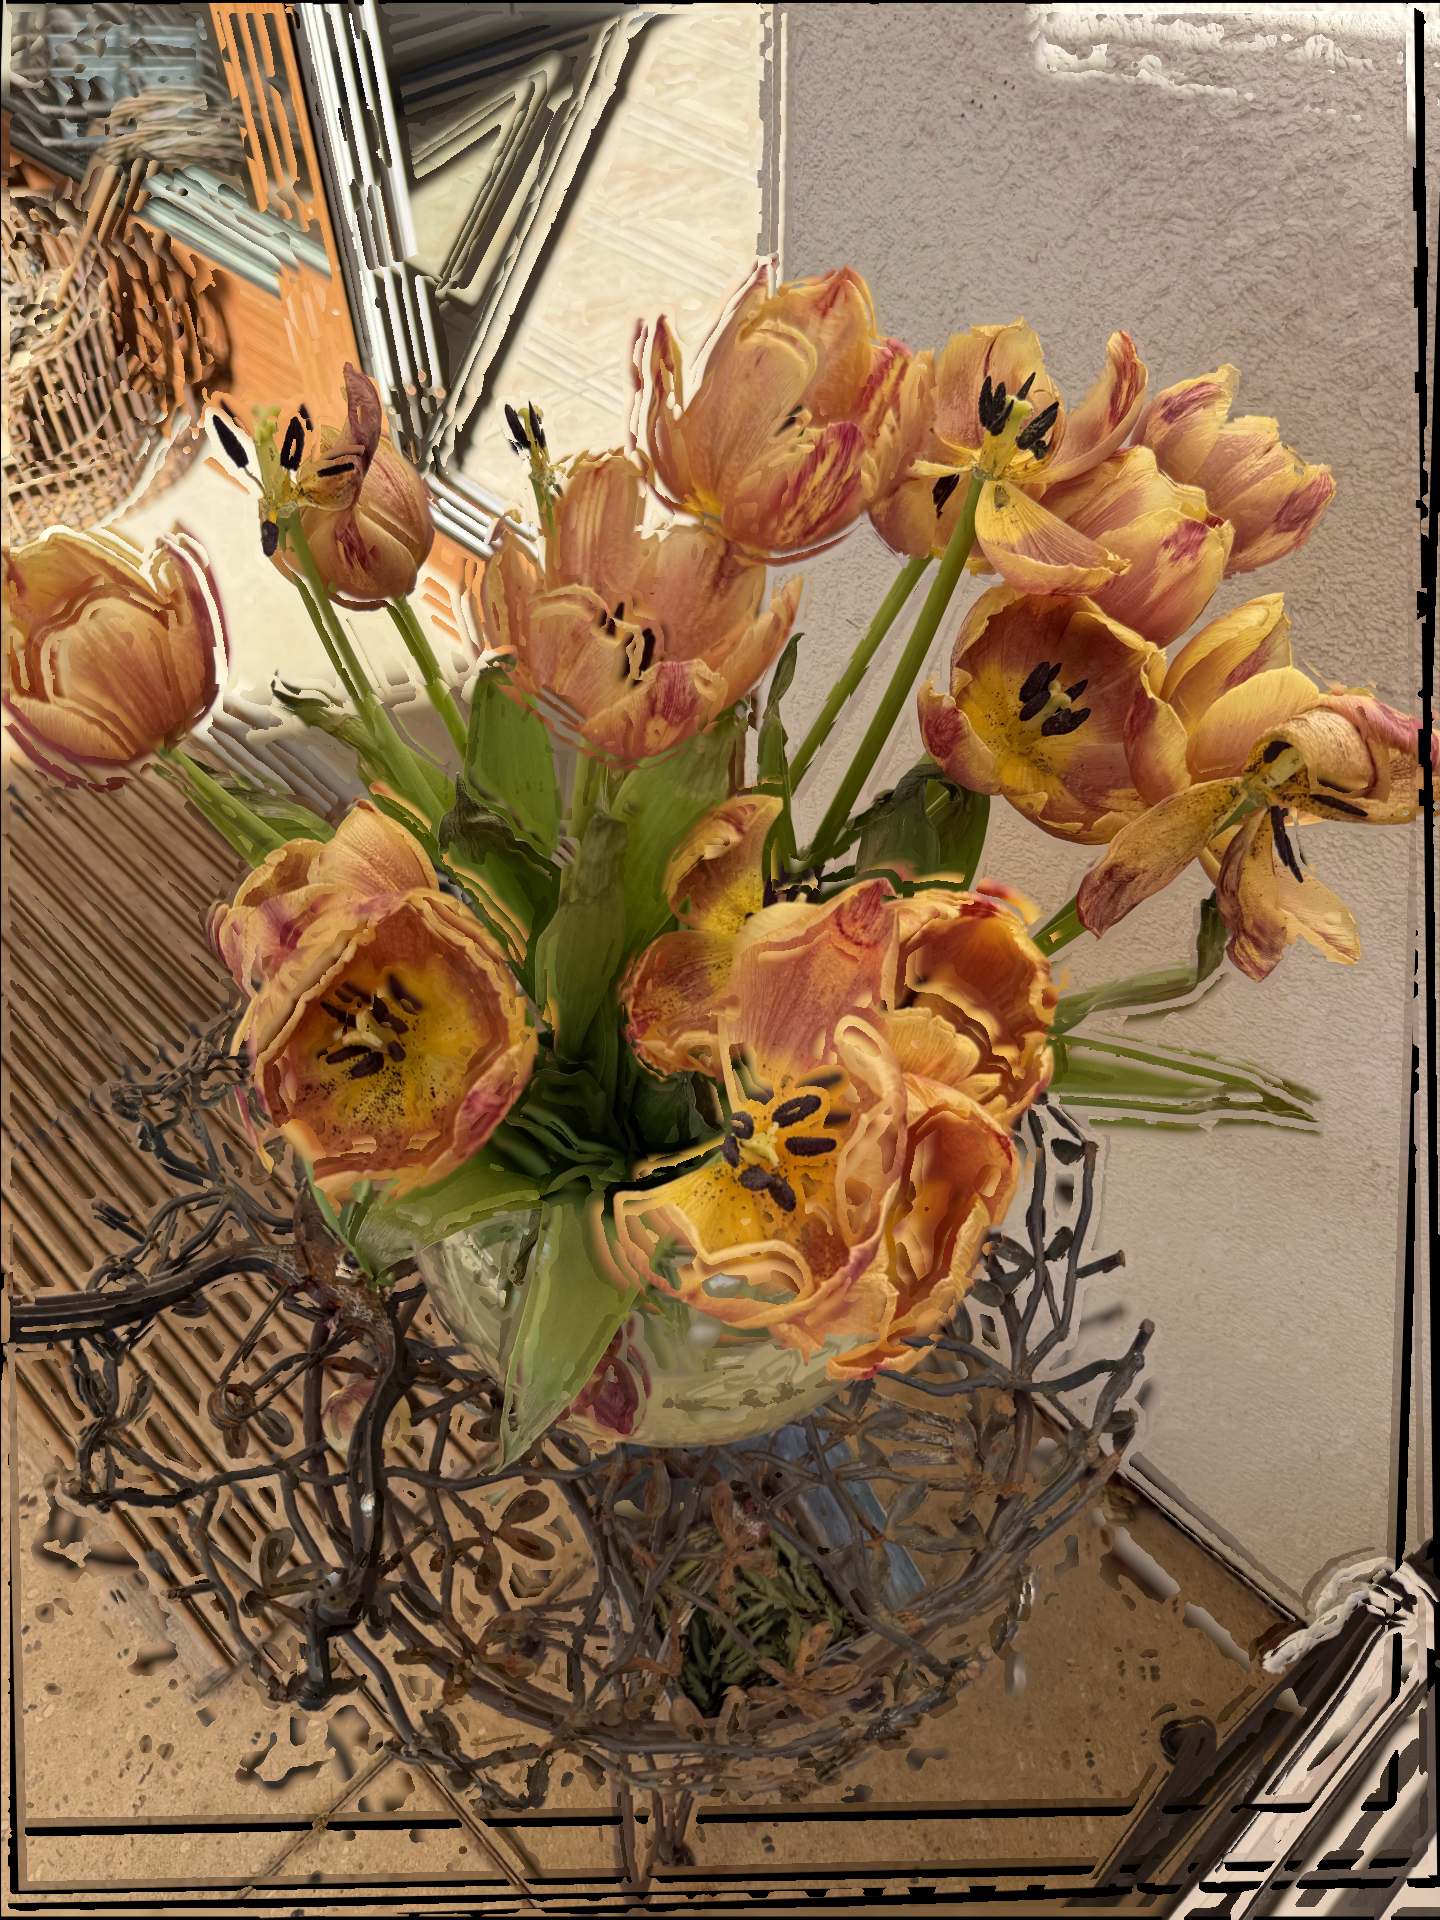
\includegraphics[width=\linewidth]{flower_fused_wta.png}
  \caption*{(b) Winner-Takes-All}
\end{minipage}\hfill
\begin{minipage}{0.24\textwidth}
  \centering
  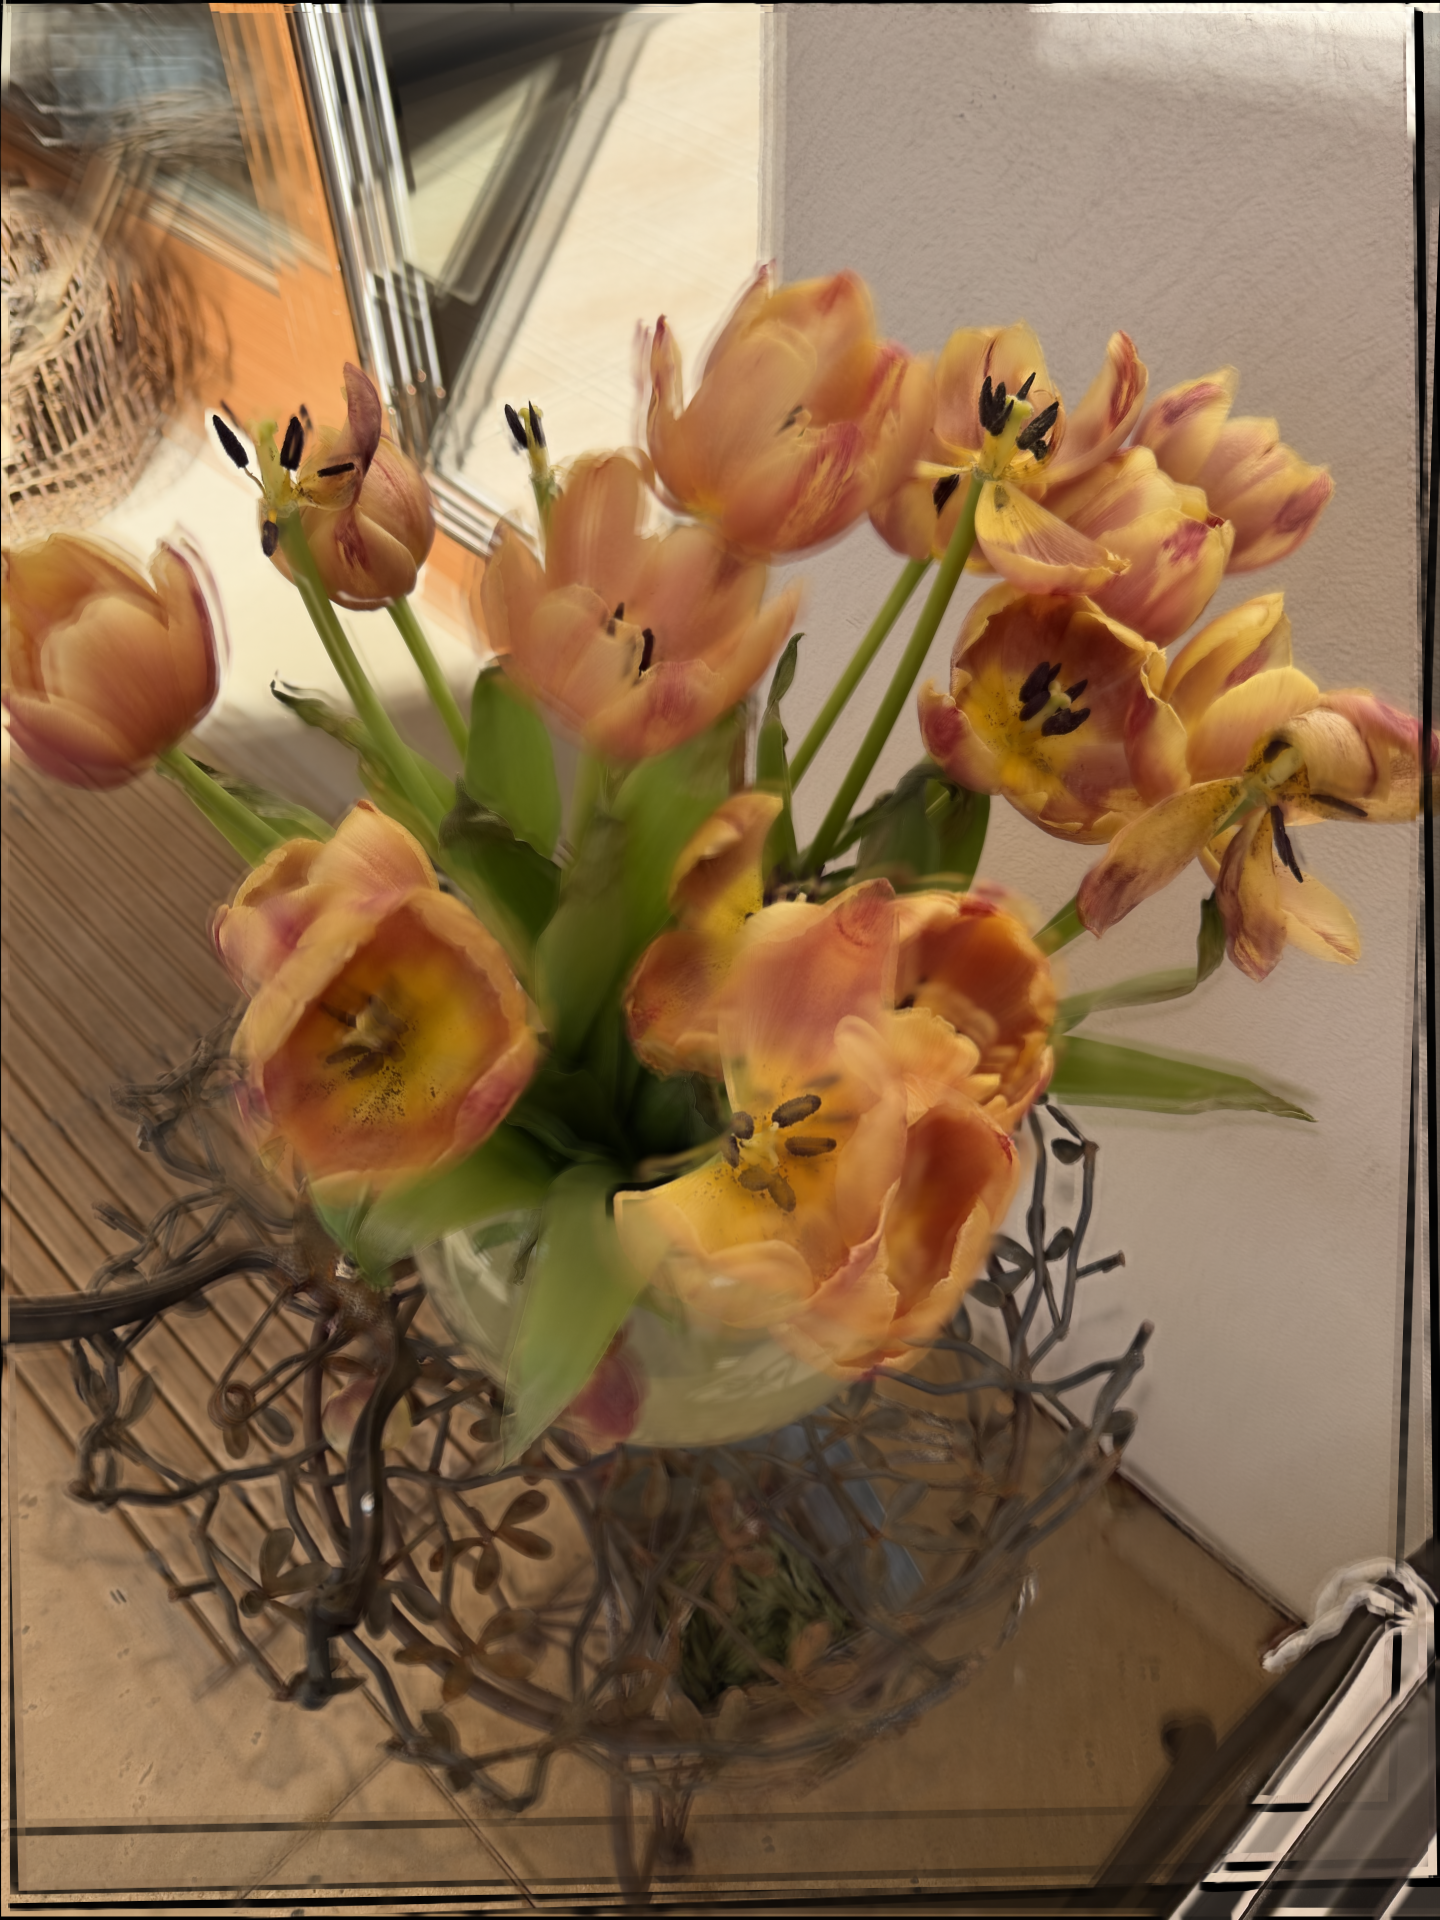
\includegraphics[width=\linewidth]{flower_fused_soft.png}
  \caption*{(c) Soft (softmax)}
\end{minipage}\hfill
\begin{minipage}{0.24\textwidth}
  \centering
  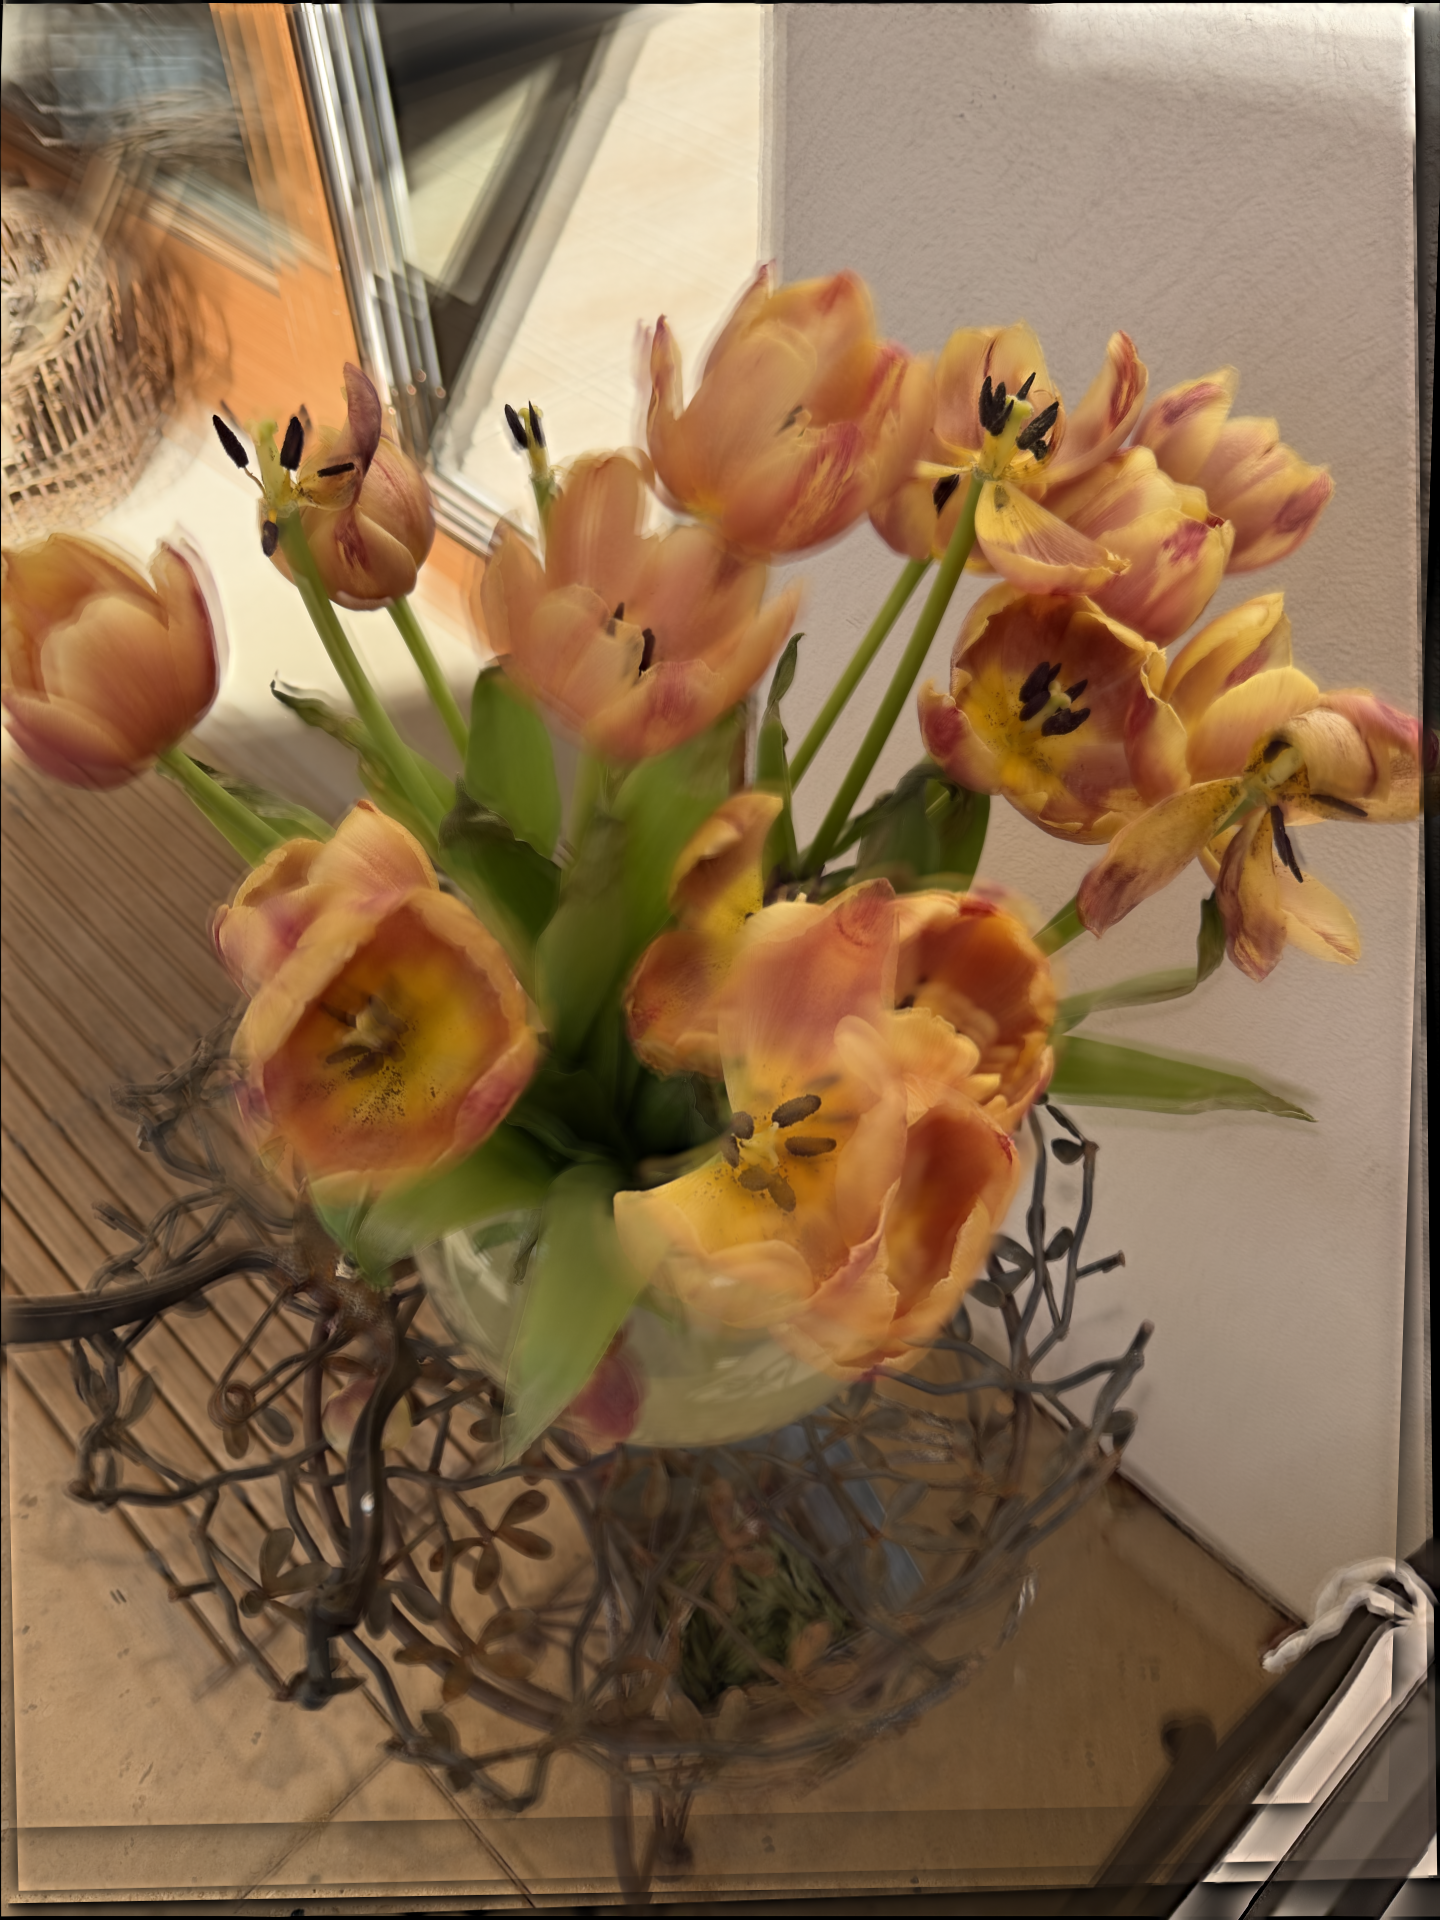
\includegraphics[width=\linewidth]{flower_fused_pyramid.png}
  \caption*{(d) Laplacian pyramid}
\end{minipage}
\caption{Flower stack (6 frames, iPhone 17 Pro Max ProRAW, $1920\times1440$). The focus map shows an ordered gradient from front petal to background, with no single frame contributing more than 28\% of pixels. WTA Tenengrad: 0.232 vs.\ single-frame 0.070.}
\label{fig:flower}
\end{figure*}

The focus map contribution is well distributed across all six frames (9--28\%), confirming a smooth focal sweep rather than a dominant frame. Pyramid blending achieves the best SSIM (0.605) while WTA gives the sharpest result (0.232).

\subsection{Insect Stack Results}

The insect stack is the most challenging dataset: three frames, subject motion between shots, and inconsistent frame dimensions resolved by center-cropping. Fig.~\ref{fig:insect} shows the results.

\begin{figure*}[t]
\centering
\begin{minipage}{0.24\textwidth}
  \centering
  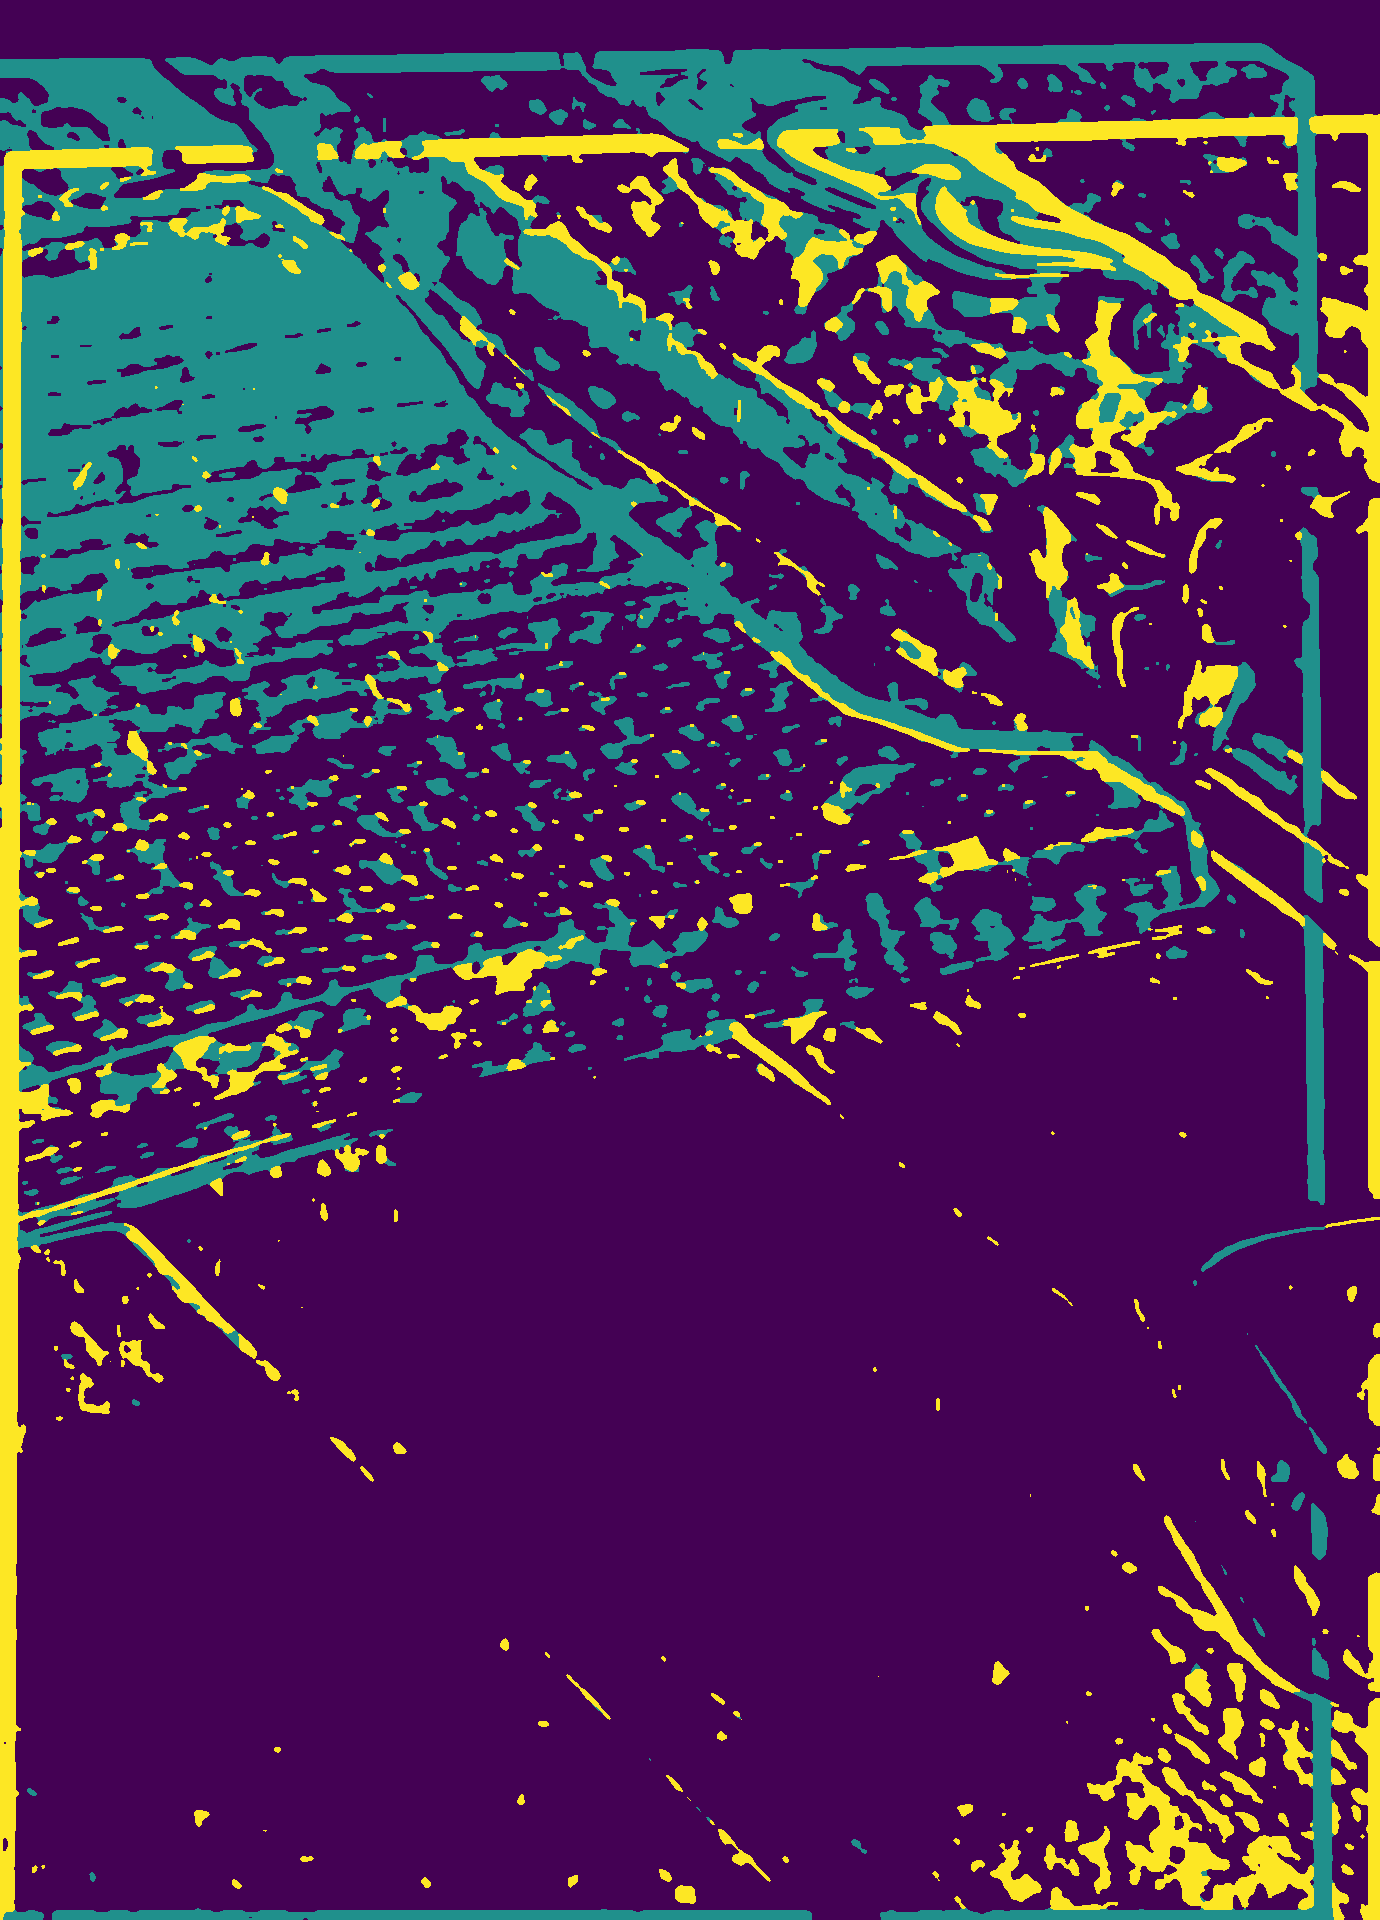
\includegraphics[width=\linewidth]{insect_focus_map.png}
  \caption*{(a) Focus map}
\end{minipage}\hfill
\begin{minipage}{0.24\textwidth}
  \centering
  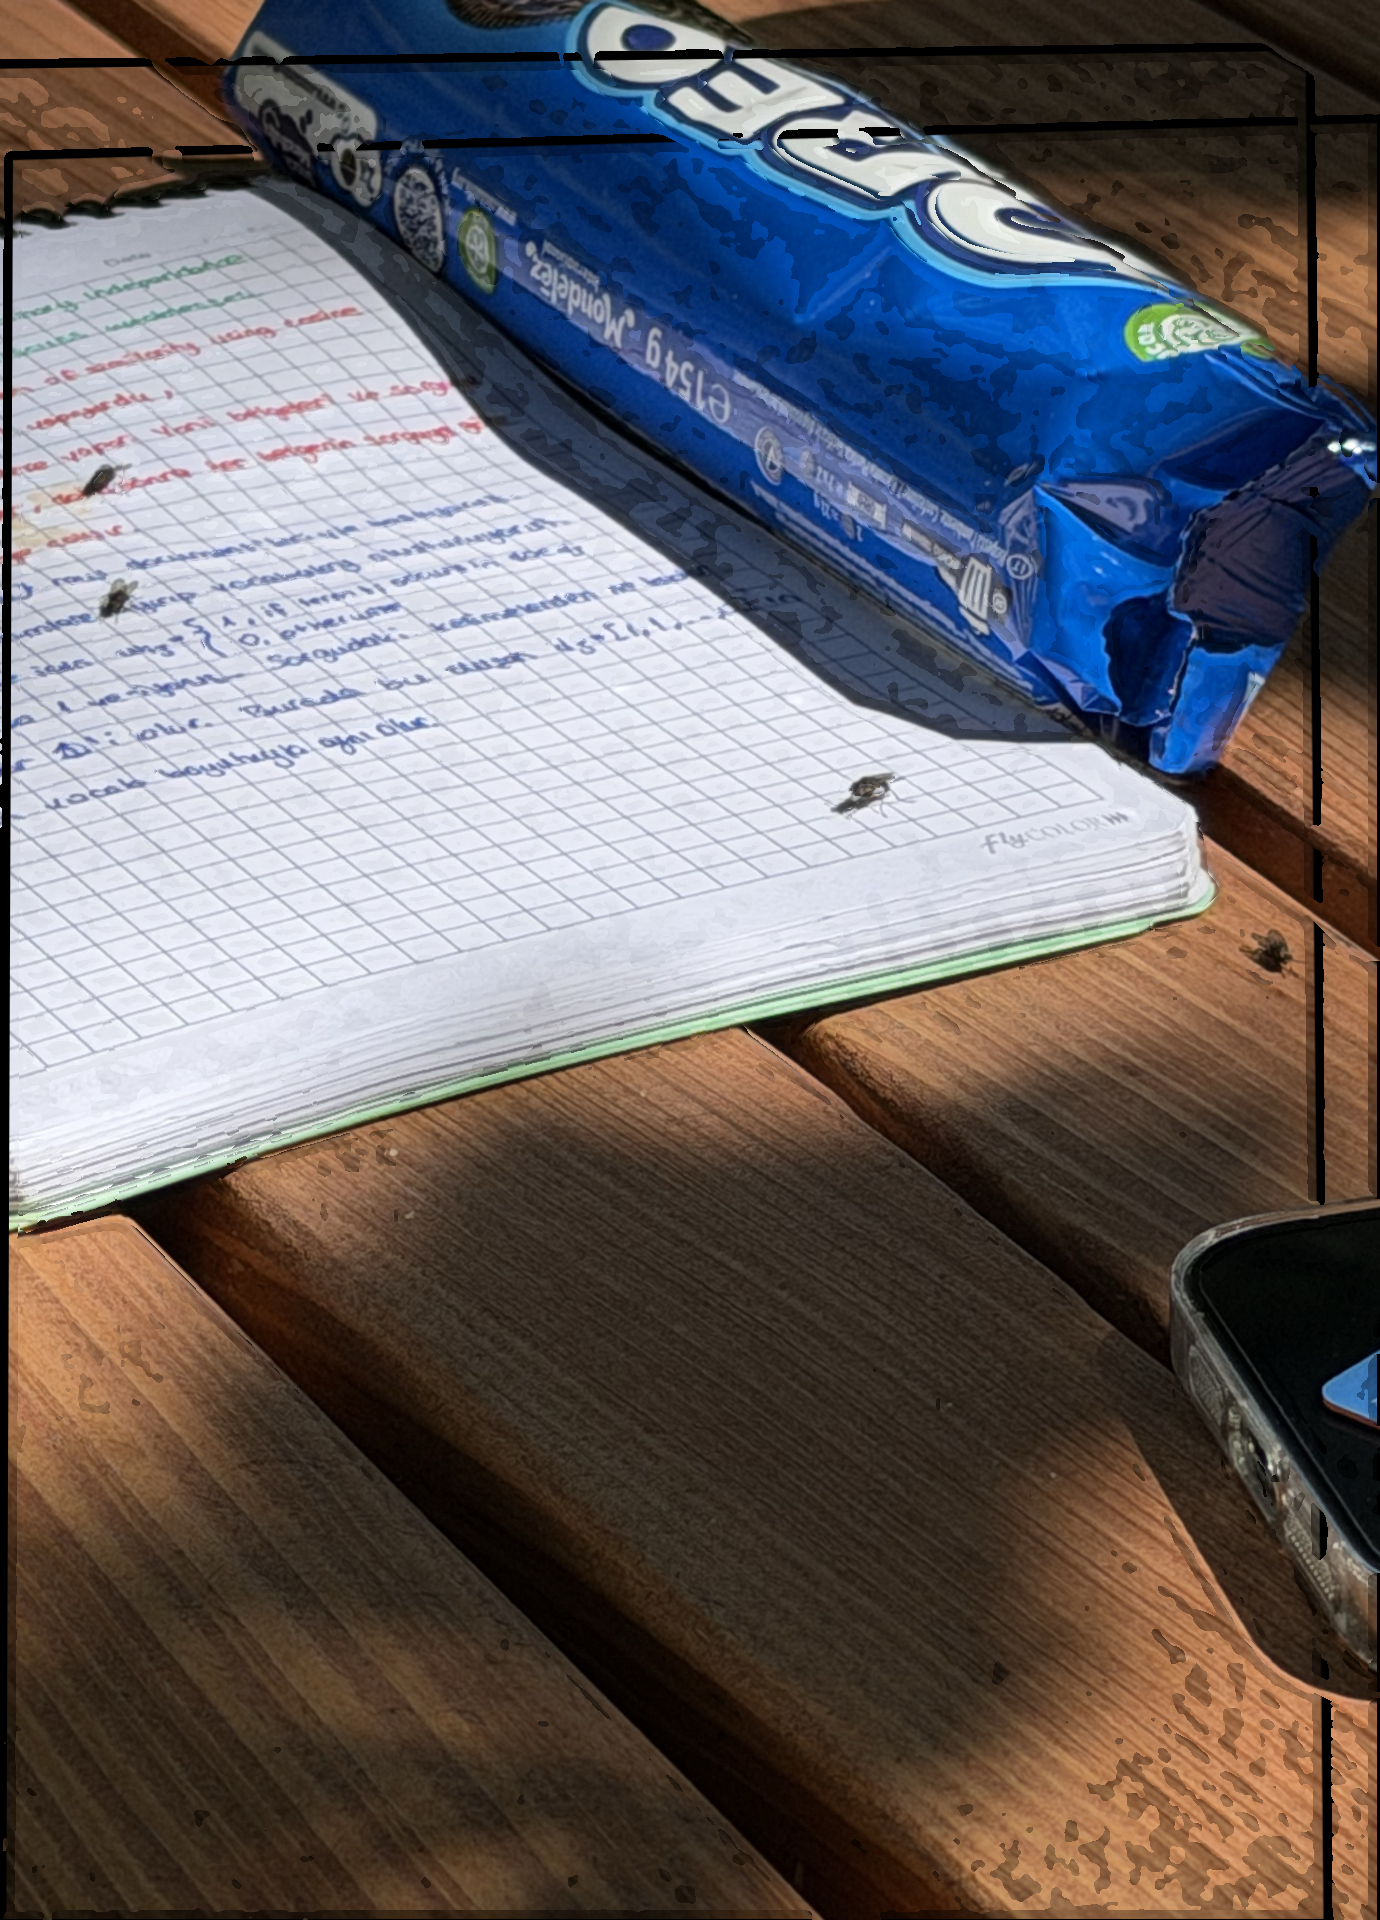
\includegraphics[width=\linewidth]{insect_fused_wta.png}
  \caption*{(b) Winner-Takes-All}
\end{minipage}\hfill
\begin{minipage}{0.24\textwidth}
  \centering
  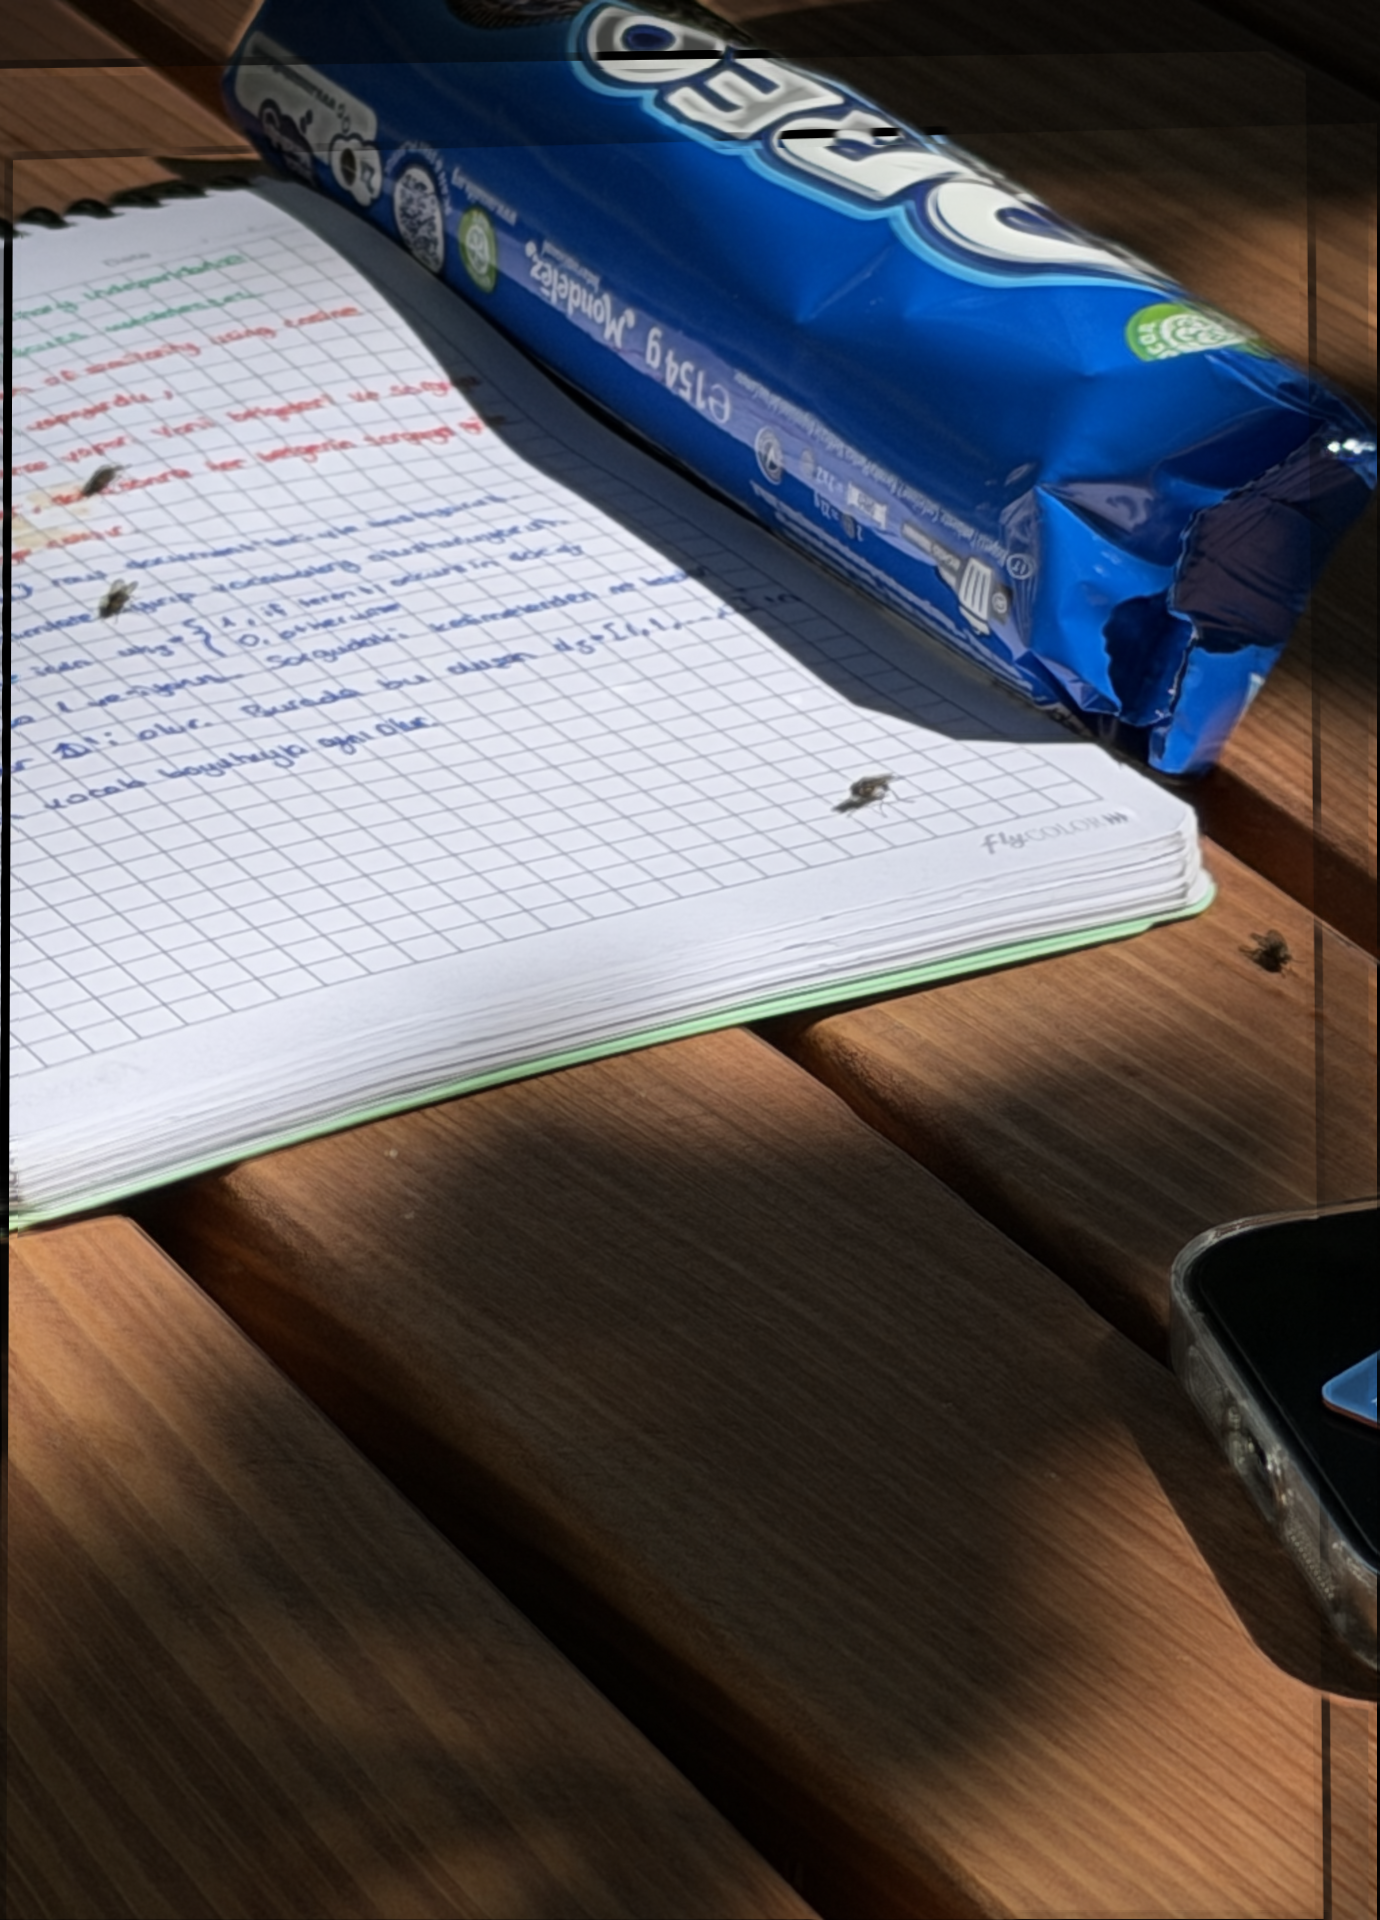
\includegraphics[width=\linewidth]{insect_fused_soft.png}
  \caption*{(c) Soft (softmax)}
\end{minipage}\hfill
\begin{minipage}{0.24\textwidth}
  \centering
  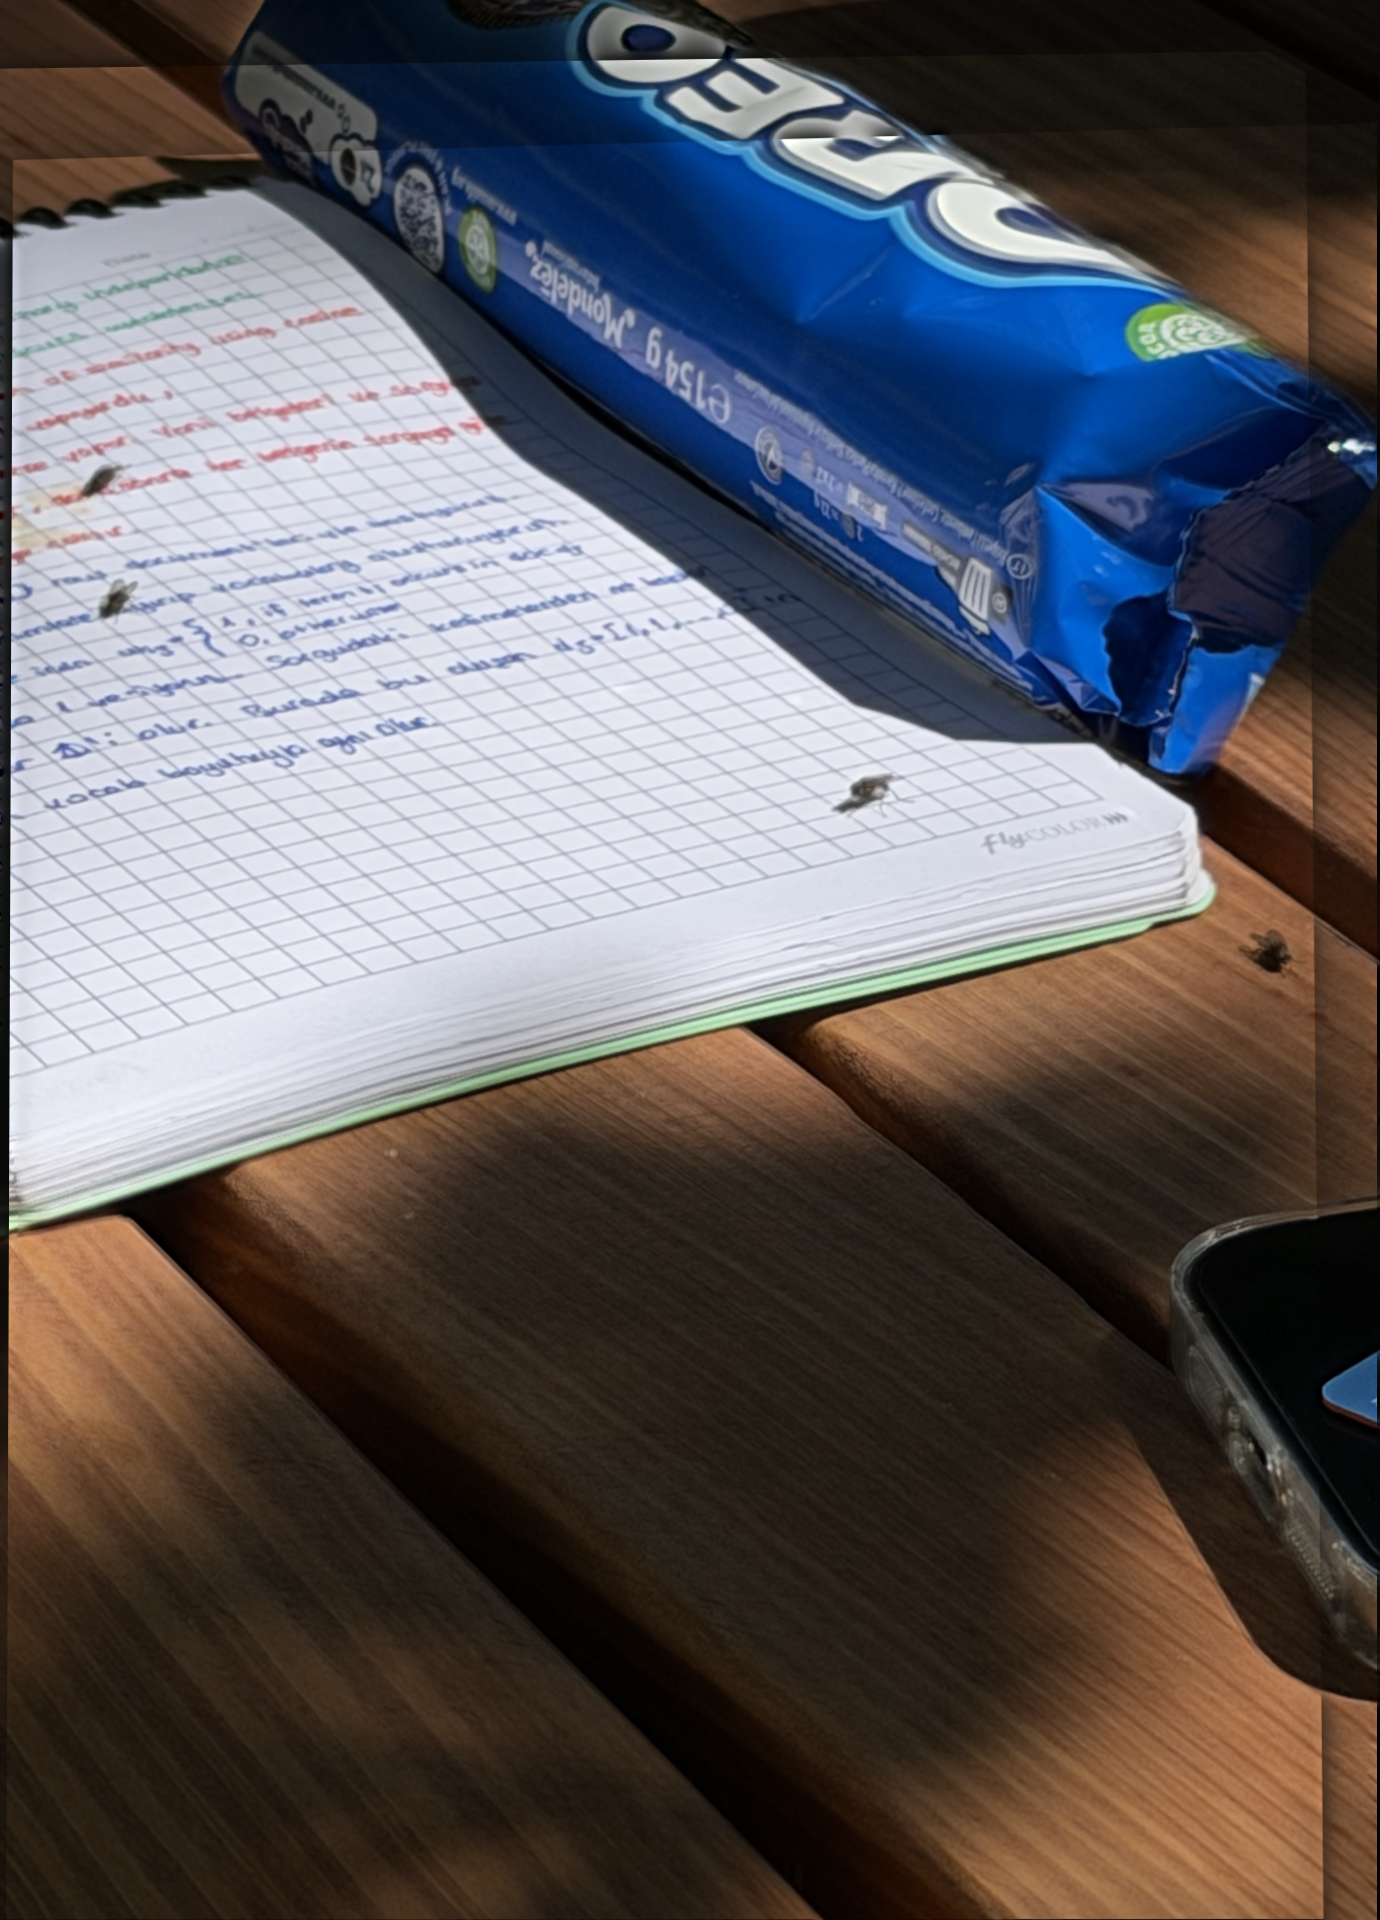
\includegraphics[width=\linewidth]{insect_fused_pyramid.png}
  \caption*{(d) Laplacian pyramid}
\end{minipage}
\caption{Insect stack (3 frames, hand-held, ECC-aligned, $1920\times1380$). Frame 0 dominates the focus map (60\%), since the insect moved between shots. Despite subject motion, WTA improves Tenengrad sharpness from 0.057 to 0.128 ($+$124\%).}
\label{fig:insect}
\end{figure*}

\textbf{Focus map distribution.} Table~\ref{tab:focus_map} shows the per-frame contribution across all datasets. For the insect stack, frame\_000 dominates (60\%) because the insect moved after the first shot, leaving frames 1--2 contributing mostly background texture. Nevertheless, the non-trivial contributions from frames 1 (15.8\%) and 2 (24.0\%) demonstrate that fusion still draws usable focused content from each frame.

\begin{table}[h]
\centering
\caption{Focus-map source percentages per stack.}
\label{tab:focus_map}
\begin{tabular}{llr}
\toprule
Dataset & Frame & \% pixels \\
\midrule
\multirow{6}{*}{Flower}
  & frame\_000 & 19.4 \\
  & frame\_001 &  9.2 \\
  & frame\_002 & 11.0 \\
  & frame\_003 & 23.0 \\
  & frame\_004 & 28.3 \\
  & frame\_005 &  9.1 \\
\midrule
\multirow{3}{*}{Insect}
  & frame\_000 & 60.3 \\
  & frame\_001 & 15.8 \\
  & frame\_002 & 24.0 \\
\midrule
\multirow{2}{*}{Lytro-03}
  & A (near)   & 57.4 \\
  & B (far)    & 42.6 \\
\midrule
\multirow{2}{*}{Lytro-11}
  & A (near)   & 21.4 \\
  & B (far)    & 78.6 \\
\midrule
\multirow{2}{*}{Lytro-13}
  & A (near)   & 31.8 \\
  & B (far)    & 68.2 \\
\bottomrule
\end{tabular}
\end{table}

ECC alignment compensates for camera translation between shots but cannot account for subject motion. Pyramid blending achieves the best SSIM on this dataset (0.680 vs.\ 0.649 for WTA), suggesting it handles motion-induced discontinuities more gracefully by weighting transitions across frequency bands rather than making hard pixel assignments.

\subsection{Lytro Benchmark Results}

Fig.~\ref{fig:lytro} shows the WTA-fused outputs for all three Lytro pairs. The benchmark pairs are pre-registered, so no alignment is required. Both depth planes contribute non-trivially in all three pairs (Table~\ref{tab:focus_map}), confirming that the focus map correctly separates near-focus and far-focus regions.

\begin{figure*}[t]
\centering
\begin{minipage}{0.32\textwidth}
  \centering
  
\includegraphics[width=\linewidth]{lytro_03_fused_wta.png}
  \caption*{(a) Lytro-03: child and toy}
\end{minipage}\hfill
\begin{minipage}{0.32\textwidth}
  \centering
  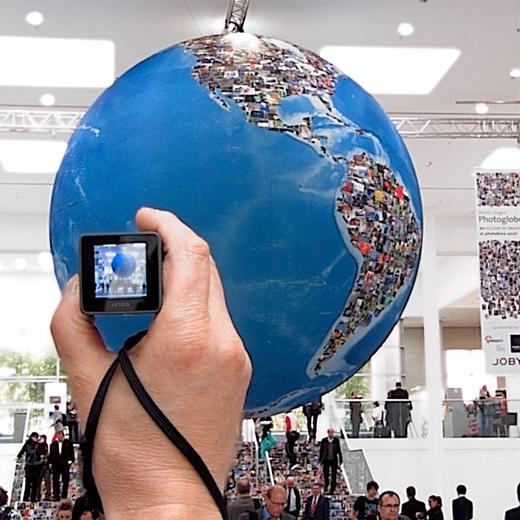
\includegraphics[width=\linewidth]{lytro_11_fused_wta.png}
  \caption*{(b) Lytro-11: camera and globe}
\end{minipage}\hfill
\begin{minipage}{0.32\textwidth}
  \centering
  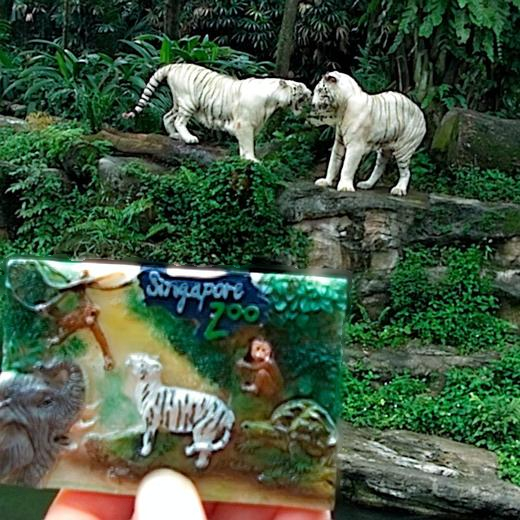
\includegraphics[width=\linewidth]{lytro_13_fused_wta.png}
  \caption*{(c) Lytro-13: zoo sign and tigers}
\end{minipage}
\caption{WTA-fused results for the three Lytro two-focus benchmark pairs. Sharpness gains: Lytro-03 $+$36\%, Lytro-11 $+$8\%, Lytro-13 $+$23\%.}
\label{fig:lytro}
\end{figure*}

Lytro-11 shows the smallest sharpness gain because both source frames already contain very high-frequency content ($\text{Ten}=0.432$ for the single best frame). Lytro-13 shows a more pronounced improvement: the zoo-sign text is sharp in one frame and the tiger is sharp in the other, making fusion meaningful.

%------------------------------------------------------------
\section{Optional Extension: Tiny Learned Focus-Scorer}

As an exploratory extension, a lightweight MLP was trained on pseudo-labels from the classical Tenengrad focus map. Table~\ref{tab:mlp_config} summarises the network configuration.

\begin{table}[h]
\centering
\caption{Tiny MLP configuration.}
\label{tab:mlp_config}
\begin{tabular}{ll}
\toprule
Hyperparameter & Value \\
\midrule
Input features     & 3 (per-pixel Tenengrad scores, normalised) \\
Hidden layers      & $2 \times 64$ units, ReLU \\
Output             & Softmax over $N$ frames \\
Pseudo-labels      & Classical Tenengrad focus map \\
Training epochs    & 140 \\
Validation accuracy& 81.2\% \\
\bottomrule
\end{tabular}
\end{table}

The network takes a 3-element feature vector (per-pixel Tenengrad scores across three selected frames, normalised) and outputs a frame probability vector. The network is implemented entirely in NumPy; no deep-learning framework is required. Fig.~\ref{fig:neural} compares the classical and neural focus maps on the plants stack.

\begin{figure}[h]
\centering
\begin{minipage}{0.48\linewidth}
  \centering
  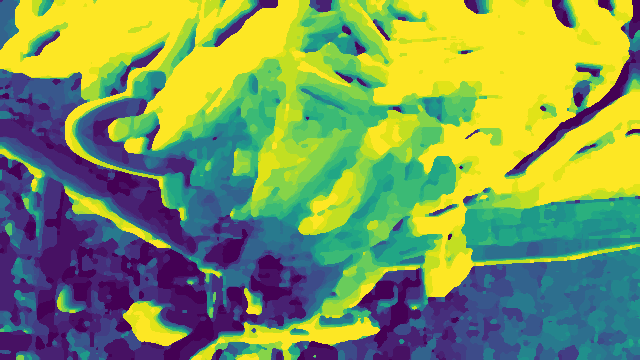
\includegraphics[width=\linewidth]{focus_map.png}
  \caption*{(a) Classical focus map}
\end{minipage}\hfill
\begin{minipage}{0.48\linewidth}
  \centering
  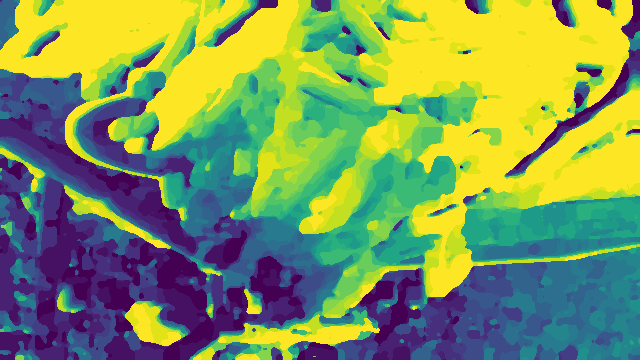
\includegraphics[width=\linewidth]{neural_focus_map.png}
  \caption*{(b) Neural focus map}
\end{minipage}
\caption{Classical Tenengrad focus map vs.\ learned MLP focus map on the plants stack. The two maps agree on 81.2\% of pixels.}
\label{fig:neural}
\end{figure}

Table~\ref{tab:neural} compares the fusion quality of the neural and classical approaches.

\begin{table}[h]
\centering
\caption{Neural vs.\ classical fusion on the plants stack.}
\label{tab:neural}
\begin{tabular}{lccc}
\toprule
Method & Tenengrad & SSIM & Entropy \\
\midrule
Classical WTA    & 0.1049 & 0.764 & 7.237 \\
Neural WTA       & \textbf{0.1050} & 0.763 & 7.238 \\
Neural soft      & 0.0967 & \textbf{0.783} & 7.225 \\
\bottomrule
\end{tabular}
\end{table}

The neural WTA is virtually identical to the classical WTA ($<$0.1\% difference in Tenengrad), expected since the network was trained on the same pseudo-labels. Neural soft blending achieves a slightly better SSIM than classical WTA (0.783 vs.\ 0.764) while remaining below pyramid blending (0.903), suggesting that learned weights provide a smoother transition field than hard argmax selection. The key observation is that a simple learned module can replicate the classical focus map without hand-crafting focus rules, pointing toward a natural extension for cases where classical measures fail (e.g., diffuse textures, chromatic defocus)~\cite{liu2017multifocus}.

%------------------------------------------------------------
\section{Conclusion}

This project demonstrates that a fully classical focal-stack pipeline—Tenengrad focus scoring, focus-map smoothing, and multi-scale fusion—reliably produces all-in-focus composites across datasets ranging from a tripod-captured plants stack to hand-held smartphone close-up and macro photography. The key findings are:

\begin{enumerate}
  \item Tenengrad (Sobel gradient energy) is the most effective focus measure among the four tested, and its ranking relative to competitors is stable across two independent datasets (plants and Lytro).
  \item Winner-takes-all fusion maximises sharpness (up to $+$233\% over the best single frame for the flower stack) but degrades SSIM; Laplacian pyramid blending provides the best structural-similarity--sharpness trade-off.
  \item ECC alignment successfully mitigates camera shake in handheld stacks but cannot compensate for subject motion; pyramid blending is more robust than WTA in the subject-motion case (insect: SSIM 0.680 vs.\ 0.649).
  \item A tiny MLP trained on classical pseudo-labels reproduces the classical focus map with 81\% pixel accuracy, confirming the feasibility of a learned focus-scorer as a future extension.
\end{enumerate}

Future work could extend the pipeline with subject-motion segmentation, optical flow alignment for moving subjects, and learning-based focus measures trained on real-world depth-annotated macro datasets.

%------------------------------------------------------------
\begin{thebibliography}{00}

\bibitem{nayar1994shape}
S.~K.~Nayar and Y.~Nakagawa, ``Shape from focus,''
\textit{IEEE Trans.\ Pattern Anal.\ Mach.\ Intell.}, vol.~16, no.~8, pp.~824--831, 1994.

\bibitem{krotkov1988focusing}
E.~Krotkov, ``Focusing,''
\textit{Int.\ J.\ Comput.\ Vis.}, vol.~1, pp.~223--237, 1988.

\bibitem{pertuz2013analysis}
S.~Pertuz, D.~Puig, and M.~A.~Garcia, ``Analysis of focus measure operators for shape-from-focus,''
\textit{Pattern Recognit.}, vol.~46, no.~5, pp.~1415--1432, 2013.

\bibitem{santos1997evaluation}
A.~Santos, C.~Ortiz de Sol\'orzano, J.~J.~Vaquero, J.~M.~Pe\~na, N.~Malpica, and F.~del Pozo, ``Evaluation of autofocus functions in molecular cytogenetic analysis,''
\textit{J.\ Microscopy}, vol.~188, no.~3, pp.~264--272, 1997.

\bibitem{burt1983multiresolution}
P.~J.~Burt and E.~H.~Adelson, ``A multiresolution spline with application to image mosaics,''
\textit{ACM Trans.\ Graph.}, vol.~2, no.~4, pp.~217--236, 1983.

\bibitem{nejati2015multi}
M.~Nejati, S.~Samavi, and S.~Shirani, ``Multi-focus image fusion using dictionary-based sparse representation,''
\textit{Inf.\ Fusion}, vol.~25, pp.~72--84, 2015.

\bibitem{evangelidis2008parametric}
G.~D.~Evangelidis and E.~Z.~Psarakis, ``Parametric image alignment using enhanced correlation coefficient maximization,''
\textit{IEEE Trans.\ Pattern Anal.\ Mach.\ Intell.}, vol.~30, no.~10, pp.~1858--1865, 2008.

\bibitem{subbarao1998optimal}
M.~Subbarao and J.-K.~Tyan, ``Selecting the optimal focus measure for autofocusing and depth-from-focus,''
\textit{IEEE Trans.\ Pattern Anal.\ Mach.\ Intell.}, vol.~20, no.~8, pp.~864--870, Aug.\ 1998.

\bibitem{zhang1999categorization}
Z.~Zhang and R.~S.~Blum, ``A categorization of multiscale-decomposition-based image fusion schemes with a performance study for a digital camera application,''
\textit{Proc.\ IEEE}, vol.~87, no.~8, pp.~1315--1326, Aug.\ 1999.

\bibitem{wang2004ssim}
Z.~Wang, A.~C.~Bovik, H.~R.~Sheikh, and E.~P.~Simoncelli, ``Image quality assessment: From error visibility to structural similarity,''
\textit{IEEE Trans.\ Image Process.}, vol.~13, no.~4, pp.~600--612, Apr.\ 2004.

\bibitem{shannon1948}
C.~E.~Shannon, ``A mathematical theory of communication,''
\textit{Bell Syst.\ Tech.\ J.}, vol.~27, no.~3, pp.~379--423, Jul.\ 1948.

\bibitem{liu2017multifocus}
Y.~Liu, X.~Chen, H.~Peng, and Z.~Wang, ``Multi-focus image fusion with a deep convolutional neural network,''
\textit{Inf.\ Fusion}, vol.~36, pp.~191--207, 2017.

\bibitem{szeliski2010}
R.~Szeliski, \textit{Computer Vision: Algorithms and Applications}.
Springer, 2010.

\end{thebibliography}

\end{document}
